\section{Технологический раздел}

% NOTE:
% Технологический раздел содержит обоснованный выбор средств программной реализации, описание основных (нетривиальных) моментов разработки и методики тестирования созданного ПО
% В этом же разделе описывается информация, необходимая для сборки и запуска разработанного ПО, форматы входных, выходных и конфигурационных файлов (если они имеются), а также интерфейс пользователя и руководство пользователя
% Часть технологического раздела должна быть посвящена тестированию разработанного ПО
% Модульное тестирование описывается в технологическом разделе
% Системное тестирование может быть описано в технологическом или исследовательском разделах

% Рек. Объем 20-25 страниц

\subsection{Выбор средств реализации}

% Обосновать выбор программных средств реализации предложенного метода

\subsection{Реализация программного обеспечения}

% Описать формат входных и выходных данных

\subsection{Результаты тестирования}

% Реализовать предложенный метод

\subsection{Пользовательский интерфейс}

% Описать взаимодействие пользователя с программным обеспечением

\subsection{Руководство пользователя}

\subsection*{Вывод}

% \section{Функциональное тестирование}
%
% В ходе работы программы, создаются три разметки:
% \begin{enumerate}
%     \item Первичная разметка --- сегмент текста классифицируется на основе анализа распределения пикселей в смежных строках, и переходов состояний в конечном автомате. Размеченный сегмент получает класс в соответствии с последним состоянием, в котором он находился. Буквально класс равен последнему состоянию.
%     \item Уточненная разметка --- класс сегмента уточняется на основе признаков самого сегмента целиком (таких как размер, количество сплошных черных участков, количество цветных строк, тепловая карта черных пикселей и т.д.). В результате сегмент получает конечный класс (Фон, Текст, Таблица, Листинг, Рисунок, График, Схема и т.д.).
%     \item Объединение сегментов --- сегменты объединяются по определенным правилам, например, небольшой фоновый или неопределенный сегмент сливается с наибольшим соседним.
% \end{enumerate}
%
% В связи с чем для проверки работоспособности программы нужно проверять корректность разметки, сформированной в конце каждого этапа отдельно для лучшей локализации возможных ошибок.
%
% % Далее будет более подробно рассмотрено тестирование программы на каждом из этапов.
% Далее будет более подробно рассмотрено тестирование программы на этапе первичной разметки.
%
% \newpage
%
% \subsection{Тестирование первичной разметки}
%
% Первичная разметка зависит от двух факторов:
% \begin{enumerate}
%     \item Точность классификации отдельной строки пикселей;
%     \item Корректность работы конечного автомата состояний.
% \end{enumerate}
%
% Таким образом, ошибка в первичной разметке сводится к некорректной классификации строки сегмента и/или некорректной работе конечного автомата состояний.
%
% Точность классификации отдельной строки пикселей зависит от:
% \begin{itemize}
%     \item Корректности правил классификации строки на основе анализа распределения пикселей в ней;
%     \item Внутренних настраиваемых параметров (например, какую строку черных пикселей считать большой или средней длины, или какие расстояния между кластерами не фоновых пикселей считать маленькими, а какие большими).
% \end{itemize}
%
% Корректность работы конечного автомата состояний зависит от корректности таблицы переходов его состояний.
%
% Правила классификации строк, значения параметров и таблица переходов состояний конечного автомата задаются либо <<на глаз>> (параметр изменяется пока разметка не станет визуально корректной), либо исходя из логических соображений (например, если в строке много черных и белых переходов, вероятно это текст, или если на предыдущем этапе сегмент был классифицирован как <<Немного текста>>, а текущая строка как <<Много текста>>, то вероятно сегмент относится к классу <<Много текста>>).
%
% Следовательно, так как работа алгоритма зависит исключительно от интуитивно подобранных правил и значений, то и корректность его работы можно оценить тоже только <<на глаз>>, например, сравнивая разметку с эталонной.
%
% % \begin{figure}[H]
% % 	\centering
% % 	\includegraphics[width=0.5\textwidth]{diag/fsm.pdf}
% % 	\caption{Конечный автомат состояний.
% %     FEW $\equiv$ <<Немного текста>>,
% %     UNDEF $\equiv$ <<Неопределено>>,
% %     MANY $\equiv$ <<Много текста>>,
% %     MBL $\equiv$ <<Средняя черная строка>>,
% %     LBL $\equiv$ <<Длинная черная строка>>,
% %     COLOR $\equiv$ <<Цвет>>}
% % 	\label{fig:fsm}
% % \end{figure}
%
% \subsubsection{Алгоритм тестирования}
%
% На рисунке ниже приведен пример алгоритма сравнения разметки с эталонной.
%
% \begin{figure}[H]
% 	\centering
% 	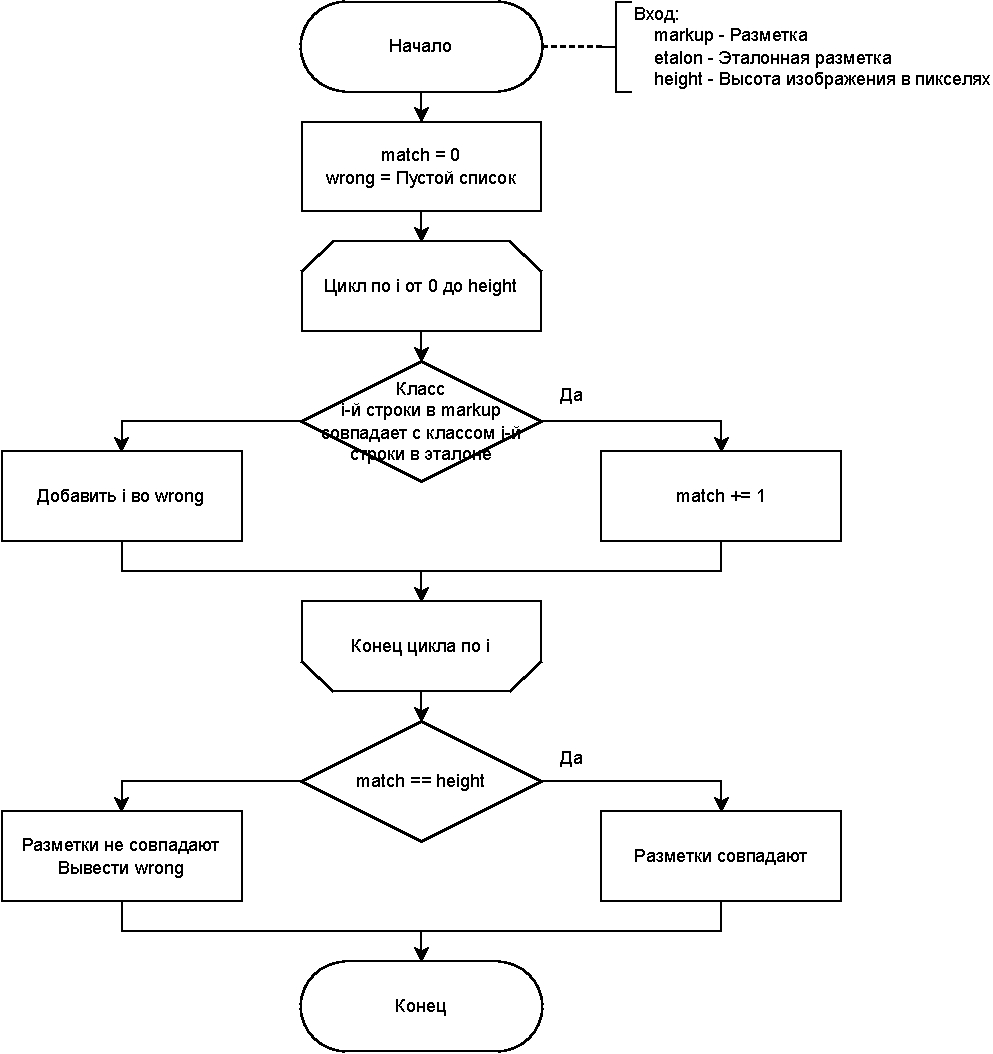
\includegraphics[width=\textwidth]{diag/vkr-test-primary.pdf}
%     \caption{Алгоритм сравнения разметки с эталонной}
% 	\label{fig:}
% \end{figure}
%
% \subsubsection{Классы эквивалентности}
%
% Классы эквивалентности естественным образом соответствуют классам первичной разметки:
% \begin{itemize}
%     \item Фон;
%     \item Неопределенность;
%     \item Много текста;
%     \item Мало текста;
%     \item Большая черная линия;
%     \item Небольшая черная линия;
%     \item Цвет.
% \end{itemize}
%
% Для тестирования разметки Фона можно предложить следующие тестовые сценарии:
% \begin{itemize}
%     \item Белая строка высотой в один пиксель;
%     \item Больше одной фоновой строки подряд;
%     \item Пустая страница.
% \end{itemize}
%
% Для тестирования вывода состояния <<Много текста>> можно предложить следующие тестовые сценарии:
% \begin{itemize}
%     \item Строка текста на русском языке;
%     \item Строка текста на английском языке;
%     \item Строка текста на китайском языке;
%     \item Строка текста длиной во всю ширину документа;
%     \item Строка текста длиной больше половины документа.
% \end{itemize}
%
% Для тестирования вывода состояния <<Мало текста>> можно предложить следующие тестовые сценарии:
% \begin{itemize}
%     \item Текст <<Мало текста>>;
%     \item Текст <<аа>>;
%     \item Строка текста длиной меньше половины документа.
% \end{itemize}
%
% Для тестирования вывода состояния <<Большая черная строка>> можно предложить следующие тестовые сценарии:
% \begin{itemize}
%     \item Большая черная строка высотой в один пиксель;
%     \item Большая черная строка высотой в несколько пикселей;
%     \item Листинг кода;
%     \item Таблица;
%     \item Черно-белое изображение в рамке.
% \end{itemize}
%
% Для тестирования вывода состояния <<Небольшая черная строка>> можно предложить следующие тестовые сценарии:
% \begin{itemize}
%     \item Небольшая черная линия;
%     \item Подчеркнутый текст;
%     \item Блок схемы алгоритма;
%     \item Схема алгоритма.
% \end{itemize}
%
% Для тестирования вывода состояния <<Цвет>> можно предложить следующие тестовые сценарии:
% \begin{itemize}
%     \item Цветное изображение без рамки;
%     \item Цветной текст;
%     \item Цветной текст внутри не цветного.
% \end{itemize}
%
% Для тестирования вывода состояния <<Неопределенность>> (состояние, в котором не удалось причислить сегмент ни к одному из состояний) можно предложить следующие тестовые сценарии:
% \begin{itemize}
%     \item Граф сверточной нейронной сети без прямых линий;
%     \item Черно-белое изображение без прямых черных линий.
% \end{itemize}
%
% \subsubsection{Результаты тестирования}
% % Листинги кода, входные данные и результаты тестирования, позитивные и негативные
% % Write some code, write some test, make it fail, make it pass
%
% Эталонная разметка, учитывающая описанные ранее сценарии тестирования, приведена в приложении.
% Цвета разметки соотносятся с классами разметки следующим образом:
% \begin{itemize}
%     \item Маджента --- <<Много текста>>;
%     \item Желтый --- <<Неопределенность>>;
%     \item Зеленый --- <<Мало текста>>;
%     \item Синий --- <<Большая черная линия>>;
%     \item Красный --- <<Небольшая черная линия>>;
%     \item Циан --- <<Рисунок>>.
% \end{itemize}
%
% Ниже приведен код для сравнения разметки с эталонной.
% Разметка представляет собой массив кортежей из трех элементов: начало сегмента, конец сегмента и класс.
%
% \begin{lstlisting}[caption={Сравнение разметки с эталонной}]
% def expand_segments(segments, height, default):
%     result = [default] * height
%     for y0, y1, cls in segments:
%         if y0 < 0 or y1 >= height:
%             raise ValueError(f"Сегмент ({y0},{y1}) выходит за границы [0, {height-1}]")
%         for y in range(y0, y1 + 1):
%             result[y] = cls
%     return result
%
% def compare_segments(markup_segs, etalon_segs, height):
%     markup = expand_segments(markup_segs, height, default)
%     etalon = expand_segments(etalon_segs, height, default)
%     match = 0
%     wrong = []
%     for i in range(height):
%         if markup[i] == etalon[i]:
%             match += 1
%         else:
%             wrong.append(i)
%     if match == height:
%         print("Разметки совпадают")
%         return True, wrong
%     else:
%         print(f"Разметки не совпадают, найдено {len(wrong)} несоответствий")
%         return False, wrong
% \end{lstlisting}
%
